% Template for ICASSP-2026 paper; to be used with:
%          spconf.sty  - ICASSP/ICIP LaTeX style file, and
%          IEEEbib.bst - IEEE bibliography style file.
% --------------------------------------------------------------------------
\documentclass{article}
\usepackage{spconf}
\usepackage{amsmath,amssymb}
\usepackage{graphicx}
\usepackage{tikz}
\usetikzlibrary{arrows.meta,positioning,fit,backgrounds,calc}
\usepackage{booktabs}
\usepackage{multirow}
\usepackage[hidelinks]{hyperref}

\let\oldthebibliography\thebibliography
\renewcommand{\thebibliography}[1]{%
  \oldthebibliography{#1}%
  \setlength{\itemsep}{0pt}\setlength{\parsep}{0pt}\setlength{\parskip}{0pt}}

% Example definitions.
% --------------------
\def\x{{\mathbf x}}
\def\L{{\cal L}}
\def\x{{\mathbf x}}
\def\L{{\cal L}}
\newcommand{\Sgal}{\mathcal{S}}
\newcommand{\Egal}{\mathcal{E}}
\newcommand{\Tlist}{\mathcal{T}}
\newcommand{\qw}{q_w}
\newcommand{\dph}{d_{\mathrm{ph}}}
\newcommand{\gac}{G_{\mathrm{ac}}}
\newcommand{\gph}{G_{\mathrm{ph}}}
\newcommand{\corpA}{\textsc{ko-fin}}
\newcommand{\corpB}{\textsc{ko-med}}
\newcommand{\zhfin}{\textsc{zh-fin}}
\newcommand{\zhleg}{\textsc{zh-leg}}
\newcommand{\zhspo}{\textsc{zh-spo}}
\newcommand{\zhtec}{\textsc{zh-tec}}
\newcommand{\best}[1]{\textbf{#1}}
\usepackage{microtype}

% Title.
% ------
\title{Correcting Domain-Term ASR Errors with Acoustic Exemplar Retrieval and a Form-Similarity Constraint.}
%
% Single address.
% ---------------
\address{Korea AI Lab (K-AI Lab), South Korea}
%
% For example:
% ------------
%\address{School\\
%	Department\\
%	Address}
%
% Two addresses (uncomment and modify for two-address case).
% ----------------------------------------------------------
%\twoauthors
%  {A. Author-one, B. Author-two\sthanks{Thanks to XYZ agency for funding.}}
%	{School A-B\\
%	Department A-B\\
%	Address A-B}
%  {C. Author-three, D. Author-four\sthanks{The fourth author performed the work
%	while at ...}}
%	{School C-D\\
%	Department C-D\\
%	Address C-D}
%
\begin{document}
\ninept
%
\maketitle
%
\begin{abstract}
Automatic speech recognition is highly accurate on generic speech, but its error
rate stays disproportionately high on domain terms, because they are rare in
training data and often near-homophones of common words. Domain terms carry much
of a transcript's meaning, yet contextual biasing requires access to the decoder
and supervised adaptation often requires labelled in-domain audio. We correct such errors after
decoding, retrieving acoustic exemplars of each domain term and substituting only
when an acoustic margin and a phonetic distance agree. Galleries combine speech mined from
the recogniser's own pseudo-labels with synthetic speech; the correction decision itself uses no reference transcript. On Korean clinical and finance speech the method lowers domain-term error by 25.5\,\% and 16.5\,\% relative under Qwen3-ASR, and by 14.3\,\% and 10.7\,\% under Whisper large-v3-turbo. Full-corpus mean per-utterance CER decreases in all four settings, although character-weighted CER increases on finance speech for both recognisers. On four Mandarin domains it lowers domain-term error by 19.2--22.0\,\% relative. An ablation attributes most of the reduction to the phonetic condition, the acoustic margin contributing little once it is applied.
\end{abstract}

%
\begin{keywords}
Speech recognition, post-ASR error correction, retrieval-based correction, pseudo-labeling, acoustic exemplar retrieval, rare word recognition 
\end{keywords}
%
\section{Introduction}
\label{sec:intro}

Automatic speech recognition (ASR) systems can achieve low aggregate error rates
while remaining unreliable for domain-specific terminology. Errors in these terms
can disproportionately affect the interpretation of a transcript, particularly in
specialised settings such as clinical communication. In the Korean clinical
evaluation pool examined in this study, Whisper large-v3-turbo achieves a
character error rate (CER) of 5.1\,\%, yet misrecognises \emph{hyeollyo}
(``haematuria'') in 98.0\,\% of the 348 utterances containing the term. This
discrepancy illustrates why aggregate recognition accuracy alone is insufficient
to characterise the preservation of domain-specific information.

Existing approaches address this problem at different stages of the recognition
pipeline. Contextual biasing incorporates relevant vocabulary during decoding
through weighted finite-state transducers or neural attention mechanisms, with
scalable variants supporting large contextual
vocabularies~\cite{aleksic2015bringing,hall2015composition,pundak2018deep,%
jain2020contextual,chang2021context,le2021deep,sun2021tree}. Post-recognition
methods include language-model rescoring~\cite{shin2019effective}, generative
error correction~\cite{chen2023hyporadise,ma2023llm} and contextual spelling
correction~\cite{guo2019spelling,wang2022towards}. Rescoring selects among
recognition hypotheses, whereas generative correction can combine information
from multiple hypotheses to produce a revised transcript; other correction
models operate directly on the top hypothesis. Contextual biasing, by contrast,
requires integration with the recogniser. We examine correction using an
existing transcript, its associated audio and a domain vocabulary, without
retraining the recogniser.

Acoustic evidence has also been used in post-recognition correction.
Pundak et al.~\cite{pundak2022onthefly} retrieve audio exemplars associated with
user-provided corrections, while Wang et al.~\cite{wang2023acoustics} introduce
external acoustic attention into contextual spelling correction. Building on
these approaches, we examine two questions: how can acoustic exemplar collections
be constructed without user corrections or reference transcripts during gallery
construction, and what additional benefit does acoustic comparison
provide when candidate substitutions are already constrained by phonetic
similarity?

We investigate an exemplar-based correction framework that requires access to the
audio, a timestamped ASR hypothesis, and a domain-term list. For each word flagged
as a potential error, the framework retrieves candidate terms using acoustic
embeddings from a pretrained, fixed speech encoder. A substitution is accepted only when the
candidate satisfies both an acoustic-margin condition relative to the recognised
word and a phonetic-distance constraint. Exemplar galleries combine speech
segments mined from ASR-generated transcripts with synthetic speech produced by
text-to-speech. The correction decision does not use reference transcripts;
however, the experimental preparation uses references for term-list selection,
Korean TTS carrier construction, and threshold selection.

The contributions of this work are threefold:

\begin{enumerate}\itemsep1pt\parskip0pt
\item \textbf{An exemplar-based framework for post-recognition domain-term
      correction.} Across Korean finance and clinical speech evaluated with two
      recognisers, the framework achieves relative reductions of       10.7--25.5\,\% in missed reference-term instances, with full-corpus mean
      per-utterance CER below baseline at the selected operating points
      (Sec.~\ref{sec:main}). These headline results are evaluated in-sample.
\item \textbf{A controlled analysis of acoustic and phonetic evidence.} We
      separately evaluate acoustic-margin filtering, phonetic filtering of
      acoustically retrieved candidates, and a text-only phonetic correction
      baseline (Sec.~\ref{sec:controls}). The acoustic margin provides little
      additional benefit once the phonetic constraint is applied. The text-only
      baseline achieves larger net reductions in missed term instances, but
      increases CER on the finance corpus, revealing a trade-off between term
      recovery and overall transcription accuracy.
\item \textbf{An assessment of the method's limitations across domains and
      languages.} Across four Mandarin domains, none of the evaluated
      configurations of the proposed decision rule satisfies the requirement that
      CER remain at or below baseline (Sec.~\ref{sec:boundary}). Together with
      the Korean controls, these results identify both the conditions under which
      the framework is effective and the limitations of its acoustic decision
      criterion.
\end{enumerate}

\begin{figure*}[t]
\centering
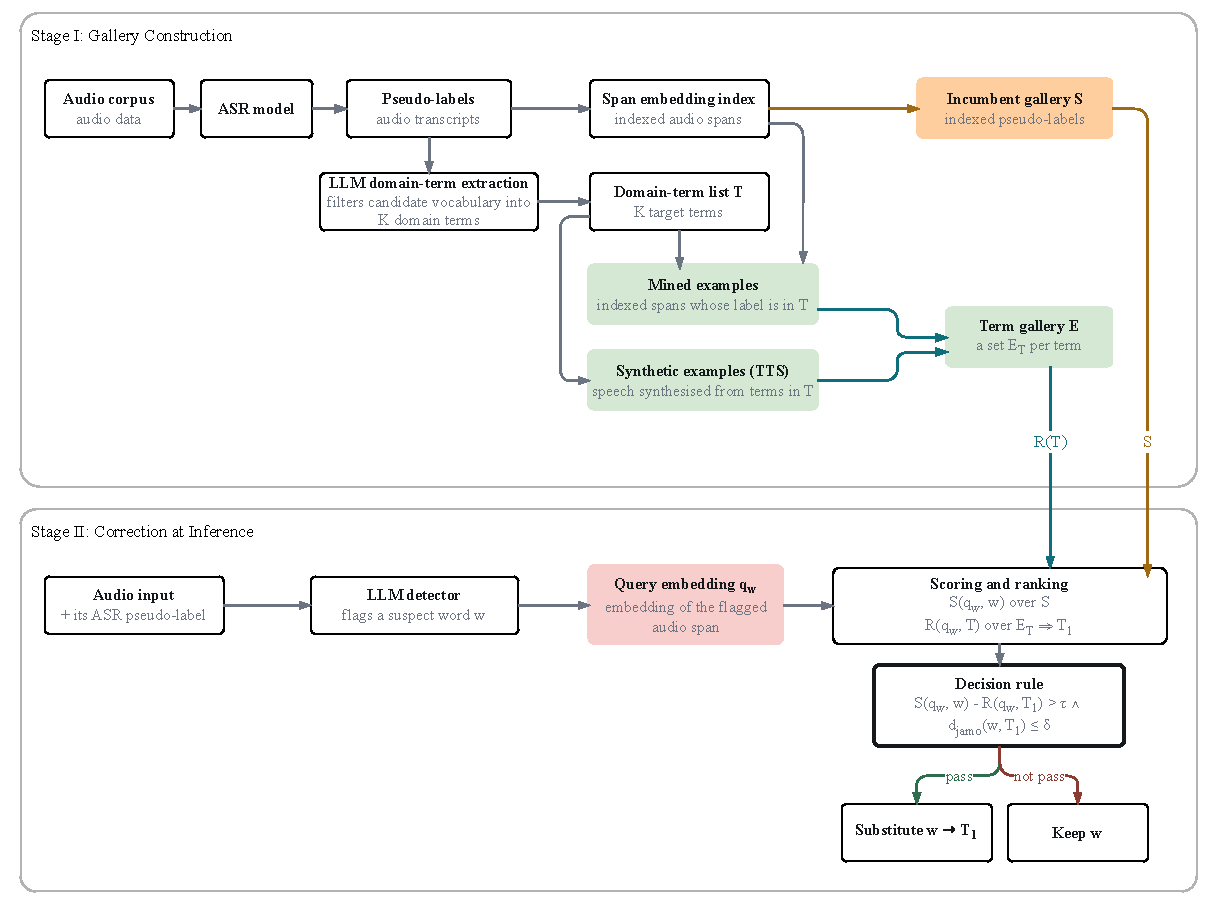
\includegraphics[width=\textwidth]{figures/fig_pipeline.pdf}
\caption{Overview of the exemplar-based correction framework. Stage~I
constructs an incumbent gallery from ASR-labelled audio spans and a domain-term
gallery from mined and synthetic exemplars. Stage~II retrieves a candidate term
for a flagged speech span and accepts the substitution only when both the
acoustic-margin and phonetic-distance conditions are satisfied. Reference text
is used during experimental preparation, including Korean TTS carrier selection,
but is not required for the correction decision.}
\label{fig:pipeline}
\end{figure*}

\section{Method}
\label{sec:method}

\subsection{Task formulation and framework overview}

We consider post-recognition correction of domain-specific terms given an audio
utterance $x$, its ASR hypothesis $h$, and a vocabulary $\Tlist$ containing $K$
target terms. A language-model-based detector identifies at most one potentially
misrecognised word $w$ in each hypothesis. The correction module then determines
whether to retain $w$ or replace it with a term from $\Tlist$.

As illustrated in Fig.~\ref{fig:pipeline}, the framework comprises two stages:
offline gallery construction and utterance-level correction. The first stage
constructs acoustic exemplar collections from ASR-labelled speech and synthesised
speech. The second stage embeds the flagged audio span, retrieves a candidate
domain term, and applies a decision rule combining acoustic and phonetic
evidence.

The correction module operates on audio and recognition hypotheses without
requiring access to decoder states, lattices, or $n$-best lists. Gallery
construction can access audio and pseudo-labels from the entire evaluation
corpus, making the acoustic indexing procedure transductive. Reference
transcripts are not required for the correction decision; however, the
experimental preparation uses references for term-list selection, Korean TTS
carrier construction, and threshold selection.

\subsection{Acoustic exemplar galleries}
\label{sec:galleries}

We extract acoustic embeddings using a pretrained HuBERT
encoder~\cite{hsu2021hubert} whose parameters remain fixed throughout the
experiments. Frame-level representations from a selected encoder layer are
averaged over time and $L_2$-normalised. The same encoder and layer are used for query spans and
gallery exemplars within each experimental configuration.

\textbf{Incumbent gallery.} The incumbent gallery $\Sgal$ contains indexed audio
spans grouped by their ASR-generated labels. For a recognised word $w$, the
subset $\Sgal_w$ therefore represents speech segments that the recogniser
transcribed as $w$. These labels are not verified against reference transcripts;
consequently, the gallery may contain systematic recognition errors.

\textbf{Domain-term gallery.} The term gallery contains an exemplar set $\Egal_T$
for each target term $T$. Exemplars are obtained from two sources. \emph{Mined
speech}: audio spans are selected when their pseudo-labels match a target term.
For terms without single-token exemplars, the Korean pipeline also searches
contiguous aligned tokens whose concatenation matches the term and embeds the
combined audio span. This procedure does not use reference transcripts to verify
the spoken content. \emph{Synthetic speech}: target terms are synthesised within
carrier sentences using multiple TTS voices. The generated sentences are aligned,
and the target-term spans are extracted and embedded using the same encoder as
the query spans.

The main Korean configuration combines mined and synthetic exemplars. Because
mining requires a matching pseudo-label span, terms that are consistently
misrecognised may have few or no mined exemplars, motivating the use of
synthetic speech to supplement their acoustic evidence. The gallery
configurations evaluated for Mandarin are specified separately in the
experimental setup.

\subsection{Query representation and acoustic retrieval}
\label{sec:gate}

For each flagged word $w$, alignment of the hypothesis to the input audio
identifies the corresponding speech span. Its normalised embedding is denoted by
$\mathbf{q}_w$. Acoustic similarity is measured using cosine distance,
$d_{\mathrm{ac}}(\mathbf{u},\mathbf{v}) = 1-\mathbf{u}^{\!\top}\mathbf{v}$.
Let $A_k$ denote the mean of the $k$ smallest available distances. The incumbent
and candidate scores are
\begin{align}
S(\mathbf{q}_w,w) &= A_{k_S}\!\left(\left\{d_{\mathrm{ac}}(\mathbf{q}_w,\mathbf{s}_i) : i\in\Sgal_w\right\}\right),
\label{eq:S}\\
R(\mathbf{q}_w,T) &= A_{k_E}\!\left(\left\{d_{\mathrm{ac}}(\mathbf{q}_w,\mathbf{e}_j) : j\in\Egal_T\right\}\right).
\label{eq:R}
\end{align}
We use $k_S=10$ and $k_E=5$. When fewer than $k$ eligible exemplars remain, the
score averages all available distances.

For each query we exclude exemplars from the same utterance to prevent self-matching. Additional speaker or session exclusions are applied according to the experimental configuration, to reduce overlap between query and gallery audio.

The candidate term is selected by
$T_1 = \arg\min_{T\in\Tlist} R(\mathbf{q}_w,T)$.
Terms without eligible exemplars are assigned an infinite retrieval score. The
hypothesis is retained when incumbent evidence is unavailable or no finite
candidate score exists. If the highest-ranked term equals $w$ or is already a
substring of $w$, the proposed substitution is discarded.

\subsection{Acoustic and phonetic decision rule}

A retrieved candidate is accepted only when it satisfies both an acoustic-margin
condition and a phonetic-distance constraint:
\begin{equation}
S(\mathbf{q}_w,w)-R(\mathbf{q}_w,T_1)>\tau
\quad\land\quad
\dph(w,T_1)\leq\delta .
\label{eq:gate}
\end{equation}
The acoustic margin compares the query's distance to the incumbent gallery with
its distance to the candidate-term gallery. A positive margin indicates that the
candidate exemplars are acoustically closer on average. The threshold $\tau$
controls the required relative advantage; a negative value permits candidates
whose retrieval score is slightly worse than the incumbent score.

The phonetic constraint restricts substitutions to terms with similar linguistic
forms. We define
\begin{equation}
\dph(w,T) = \frac{\operatorname{Lev}\!\left(\phi(w),\phi(T)\right)}
                 {\max\!\left(|\phi(w)|,|\phi(T)|,1\right)} ,
\label{eq:dph}
\end{equation}
where $\operatorname{Lev}$ is Levenshtein distance and $\phi$ maps text to a language-specific symbol sequence. For Korean, $\phi$ decomposes written Hangul syllables into jamo without applying pronunciation-conversion rules, so the distance measures orthographic form. For Mandarin, $\phi$ uses pinyin initials and finals with tone information, which makes the distance phonetic. We use \emph{phonetic} as a shorthand for both throughout.


When both conditions hold, the flagged word is replaced by $T_1$; otherwise the
original hypothesis is retained. The framework makes at most one substitution per
utterance. The contribution of each decision condition is evaluated through the
controls described in Sec.~\ref{sec:controls}.

\section{Experimental setup}
\label{sec:setup}

\subsection{Corpora and target vocabularies}
\label{sec:data}

We evaluate the method on two Korean corpora and four Mandarin domain subsets. \corpA{} comprises 59{,}054 utterances from a financial counselling subset of AI-Hub \emph{Counselling Speech}. \corpB{} comprises 51{,}898 utterances from AI-Hub \emph{Medical Staff and Patient Speech}. ASR hypotheses are generated for all utterances in both corpora.

The Mandarin data are drawn from AISHELL-1~\cite{bu2017aishell} and divided into four domain subsets: finance (\zhfin{}, 52{,}840 utterances), legal (\zhleg{}, 30{,}301), sport (\zhspo{}, 24{,}028) and technology (\zhtec{}, 19{,}765). Since AISHELL-1 does not provide domain annotations, we derive the domain split ourselves.

Each target vocabulary contains 100 terms. Candidates must occur in at least 10--20 utterances and have a recognition error rate of at least 8--10\,\%, depending on the corpus, and are ranked by recognition error. The Korean lists are additionally screened for domain relevance with Qwen3-4B-Instruct. Vocabulary selection uses reference transcripts and the corresponding recogniser's output.

We additionally explored domain-term candidate extraction from Korean ASR pseudo-labels without referring to reference transcripts during candidate generation. Tokens were analysed with Kiwi, a Korean morphological analyser~\cite{lee2024kiwi}, and filtered to remove grammatical and generic items, after which the 1{,}000 most frequent survivors were retained. A second pass then judged domain relevance, narrowing the pool to 272 candidates on \corpA{} and 295 on \corpB{} while recovering 67 and 64 of the 100 curated terms, the same coverage as the unnarrowed pool. Domain relevance was assessed manually in this exploratory experiment, and the curated vocabularies were used only to examine coverage and to guide filter refinement. Applying the same procedure to Mandarin requires word segmentation first, since pseudo-labels  carry no word boundaries. With jieba and a deeper cut of 5{,}000 candidates, the Mandarin pool narrows to 907 and recovers 50 of the 100 curated AISHELL-1 terms. This is a preliminary alternative to reference-based vocabulary selection, and the correction results reported here use the reference-selected term lists.


\subsection{Recognition systems and implementation}

Whisper large-v3-turbo~\cite{radford2023robust} is evaluated on both Korean domains and all four Mandarin domains. Qwen3-ASR-1.7B~\cite{qwen2026asr} is additionally evaluated on the Korean corpora. Each corrected transcript is compared with the original output of the same recogniser.

The encoder is HuBERT: layer 10 of \texttt{hubert-base-korean} for Korean and layer 9 of \texttt{chinese-hubert-base} for Mandarin. Frame representations are mean-pooled into 768-dimensional vectors and $L_2$-normalised. In the Korean Whisper experiments, indexed spans use Whisper's word timestamps; flagged utterances are realigned with Qwen3-ForcedAligner-0.6B~\cite{qwen2026asr} to locate query spans. Indexed spans include 0.05\,s of padding on each side. Spans shorter than 0.08\,s and single-character labels are excluded.

The Korean detector uses Gemini-3-Flash with domain-specific prompts, temperature zero, and batches of 20 utterances. Its utterance-level recall and precision are 73.8\,\% and 35.2\,\% on \corpA{}, and 89.5\,\% and 75.6\,\% on \corpB{}. For this calculation an utterance is considered erroneous if its hypothesis omits at least one reference term.

Synthetic exemplars are generated with Qwen3-TTS~\cite{qwen2026tts} using three
voices. The main experiments combine mined and synthetic exemplars for both
languages.

\subsection{Baselines and controls}

The baseline is the uncorrected output of each ASR system. On the Korean Whisper
outputs we compare the proposed decision rule with three controls:
acoustic-margin filtering alone, phonetic filtering alone, and text-only
correction. The first two retain the same acoustically retrieved candidates and
isolate the contribution of each acceptance condition. The text-only control
instead selects the vocabulary term with the smallest phonetic distance to the
flagged word and applies the phonetic threshold.

All controls use the same detector, vocabulary and evaluation pool. For the
matched comparison, text-only correction is restricted to utterances for which
the acoustic pipeline produces a candidate; its candidate selection and
acceptance decisions use no acoustic scores. Thresholds are fixed at the
corresponding Korean Whisper operating point. We compare substitution counts,
domain-term error rate and character error rate. Decoder-time contextual biasing
and trained spelling-correction models are not evaluated.

\subsection{Evaluation metrics and protocol}

We report domain-term error rate (DTER) and character error rate (CER). A term
instance is one distinct target term occurring in an utterance's reference
transcript; an instance is correct if the term appears anywhere in the
hypothesis. DTER is
\begin{equation}
\mathrm{DTER} = \frac{N_{\mathrm{missed}}}{N_{\mathrm{reference}}}\times 100\,\% ,
\label{eq:dter}
\end{equation}
where $N_{\mathrm{missed}}$ is the number of reference-term instances missing
from the hypotheses and $N_{\mathrm{reference}}$ the total number of
reference-term instances. Korean evaluation uses token-anchored matching;
Mandarin evaluation uses Han-character substring matching after orthographic
normalisation.

DTER does not penalise inserted terms absent from the reference. We therefore report CER to assess changes to the complete transcript. Main-result CER is the
mean of per-utterance CER over each full Korean corpus or Mandarin domain. Utterances without accepted substitutions retain their ASR hypotheses. For the
Korean main results, the same numeral and orthographic normalisation is applied to the original and corrected hypotheses; Mandarin uses its language-specific normalisation. We also examine micro CER, defined as total character edits divided by total reference characters.


For each corpus and recogniser, results are compared with the corresponding
uncorrected ASR output. We report the number of reference-term instances
alongside DTER because the selected vocabularies and denominators differ across
experiments. Absolute changes in error rates are expressed in percentage points.

Thresholds are selected to minimise DTER subject to CER remaining at or below
baseline, with selection restricted to the proposed joint acoustic and phonetic
rule; configurations that violate the CER condition are reported separately. In
the Korean Whisper experiments the selected phonetic threshold is
$\delta = 0.6$, with $\tau = 0$ on \corpA{} and $\tau = -0.1$ on \corpB{}.
 
The main evaluation is in-sample. Vocabulary and threshold selection use each run's original pool; the selected corrections are then rescored over the full corpus without retuning. Qwen3-ASR on \corpB{} uses the full corpus for correction; the other Korean runs use reference-selected pools. The control and grouped-split analyses retain their original pool-based scoring and normalisation. 

\begin{table}[t]
\centering
\caption{Use of reference transcripts during data preparation, correction and
evaluation.}
\label{tab:refuse}
\setlength{\tabcolsep}{3.5pt}\small
\begin{tabular}{@{}p{2.6cm}p{5.3cm}@{}}
\toprule
stage & use of reference transcripts \\
\midrule
acoustic indexing and exemplar mining & \textbf{no} -- spans are indexed and
  selected using ASR pseudo-labels \\[2pt]
Korean TTS carrier selection & \textbf{yes} -- carrier sentences are selected
  from reference transcripts \\[2pt]
error detection and correction & \textbf{no} -- references are not used to
  determine substitutions \\[2pt]
term-list selection & main experiments use reference--hypothesis discrepancies,
  with LLM screening for Korean; the exploratory alternative generates
  candidates from pseudo-labels \\[2pt]
threshold selection & references are used on the evaluation pool for the main
  results and on the development subset for the threshold-split analysis
  \\[2pt]
evaluation and domain assignment & references are used to calculate DTER and
  CER and to assign the Mandarin domain labels \\
\bottomrule
\end{tabular}
\end{table}

\noindent Once the vocabulary, galleries and thresholds have been prepared,
correction can operate without reference transcripts. The reference-selected
vocabularies prioritise error-prone terms, so their baseline DTER values should
not be interpreted as error rates over the complete vocabulary.

\section{Results}
\subsection{Main results}
\label{sec:main}

\begin{table}[t]
\centering
\caption{Korean correction results. $N_{\mathrm{ref}}$ is the number of reference-term instances. $\Delta$CER is full-corpus mean per-utterance CER change in percentage points, using common Korean normalisation.}
\label{tab:main}
\setlength{\tabcolsep}{3.4pt}\small
\begin{tabular}{llrrrr}
\toprule
 & & & \multicolumn{2}{c}{DTER (\%)} & \\
\cmidrule(lr){4-5}
corpus & ASR & $N_{\mathrm{ref}}$ & base & \best{corr.} & $\Delta$CER \\
\midrule
\multirow{2}{*}{\corpA{}}
 & Qwen3-ASR & 69{,}429 & \phantom{0}9.71 & \best{\phantom{0}8.10} & $-0.006$ \\
 & Whisper   & 53{,}270 & \phantom{0}6.12 & \best{\phantom{0}5.46} & $-0.002$ \\
\multirow{2}{*}{\corpB{}}
 & Qwen3-ASR & 39{,}586 & \phantom{0}9.30 & \best{\phantom{0}6.93} & $-0.040$ \\
 & Whisper   & 39{,}215 & 14.91 & \best{12.78} & $-0.041$ \\
\bottomrule
\end{tabular}
\end{table}

Table~\ref{tab:main} presents the selected operating point for each Korean corpus and recogniser. Correction reduces DTER in all four settings while keeping full-corpus mean per-utterance CER below baseline. Under Whisper, DTER decreases from 6.12\,\% to 5.46\,\% on \corpA{} and from 14.91\,\% to 12.78\,\% on \corpB{}; under Qwen3-ASR it decreases from 9.71\,\% to 8.10\,\% and from 9.30\,\% to 6.93\,\% respectively.

The CER reductions are small, particularly on \corpA{}, and depend on the averaging convention. On \corpA{}, micro CER increases by $+0.009$ percentage points under Qwen3-ASR and $+0.006$ under Whisper; on \corpB{} both estimators decrease. The finance results therefore do not establish improvement under character-weighted evaluation. Since the recognisers use different error-selected vocabularies, DTER comparisons should be made against the baseline within each row.


\subsection{Acoustic and phonetic controls}
\label{sec:controls}

\begin{table}[t]
\centering
\caption{Controls on Korean Whisper outputs, retaining original evaluation-pool CER and normalisation. The text-only row uses the matched candidate-utterance subset described in Sec.~\ref{sec:setup}.}
\label{tab:controls}
\setlength{\tabcolsep}{2.6pt}\small
\begin{tabular}{llrrr}
\toprule
corpus & condition & subs & \best{DTER (\%)} & $\Delta$CER \\
\midrule
\multirow{4}{*}{\corpA{}}
 & acoustic margin only     & 3{,}276 & 5.80 & $+0.327$ \\
 & phonetic constraint only & \phantom{0}917 & 5.45 & $+0.006$ \\
 & joint rule               & \phantom{0}821 & 5.46 & \best{$-0.003$} \\
 & text-only correction     & 3{,}201 & \best{5.09} & $+0.148$ \\
\midrule
\multirow{4}{*}{\corpB{}}
 & acoustic margin only     & 3{,}441 & 12.79 & $+0.799$ \\
 & phonetic constraint only & 1{,}152 & 12.78 & $-0.062$ \\
 & joint rule               & 1{,}152 & 12.78 & \best{$-0.062$} \\
 & text-only correction     & 2{,}990 & \best{11.11} & $-0.044$ \\
\bottomrule
\end{tabular}
\end{table}

Table~\ref{tab:controls} compares the acceptance conditions and the text-only
baseline on the Korean Whisper outputs. Acoustic-margin filtering alone reduces
DTER on both corpora but increases CER by 0.327 percentage points on \corpA{}
and 0.799 on \corpB{}. Acoustic proximity alone therefore provides insufficient
selectivity at these operating points.

Phonetic filtering substantially reduces the number of substitutions and their
CER cost. On \corpB{}, phonetic filtering alone and the joint rule accept
exactly the same 1{,}152 substitutions: the acoustic-margin condition provides
no additional filtering at this operating point.

On \corpA{}, adding the acoustic margin rejects 96 substitutions. This decreases
the net number of recovered term instances by 10 while improving $\Delta$CER
from $+0.006$ to $-0.003$ percentage points. The margin therefore determines
whether this configuration satisfies the CER constraint, although its effect is
small.

Text-only correction achieves lower DTER than the joint rule on both corpora. On
\corpA{} this improvement is accompanied by an increase in CER. On \corpB{} both
methods reduce CER: text-only correction recovers more reference-term instances,
while the joint rule produces the larger CER reduction. The comparison therefore
identifies a trade-off between target-term recovery and overall transcription
accuracy.

The corpora also differ in detector precision, vocabulary composition and
exemplar coverage. These experiments do not isolate the contribution of detector
precision to the observed differences.

\subsection{Incumbent-gallery analysis}
\label{sec:incumbent}

We examine whether systematic recognition errors may affect the incumbent
gallery. For each accepted substitution we calculate the proportion of eligible
incumbent exemplars whose source utterance contains the proposed term in its
reference transcript. This analysis includes only exemplar utterances with
references available in the evaluation pool.

For substitutions classified as term restorations, the median proportion is
73.2\,\% on \corpA{} and 100.0\,\% on \corpB{}. The corresponding medians are
zero for the w2w and c2w categories, and 1.9\,\% and 2.2\,\% for r2w.

These observations are consistent with systematic ASR errors contributing
related speech to the gallery of an incorrect written form. However,
reference-term presence is measured at the utterance level and does not
establish the content of each indexed span. The analysis suggests a possible
explanation for the limited contribution of the acoustic margin; it does not
establish a negative correlation between the margin and successful correction.

\subsection{Threshold-selection analysis}
\label{sec:split}

The grouped threshold-split analysis evaluates whether improvements persist when
thresholds are selected on a separate subset. On \corpA{} the selected
thresholds produce a relative DTER reduction of 10.5\,\% (95\,\% confidence
interval 8.7--12.6\,\%) and a CER change of $-0.017$ percentage points. On
\corpB{} the relative DTER reduction is 16.3\,\% (11.5--23.4\,\%) at a CER
change of $-0.078$.

Both evaluation subsets retain improvements in DTER and CER, providing evidence
that the observed reductions are not confined to the original threshold choices.
Vocabulary selection and gallery construction remain unchanged, however, so this
analysis does not provide an independent evaluation of the complete pipeline.

\subsection{Mandarin evaluation}
\label{sec:boundary}

\begin{table}[t]
\centering
\caption{Mandarin results for the proposed joint rule. Lowest DTER is selected
without a CER constraint. CER changes are in percentage points.}
\label{tab:mandarin}
\setlength{\tabcolsep}{3.0pt}\small
\begin{tabular}{lrrrrr}
\toprule
 & & \multicolumn{2}{c}{DTER (\%)} & assoc. & min \\
\cmidrule(lr){3-4}
domain & $N_{\mathrm{ref}}$ & base & lowest & $\Delta$CER & $\Delta$CER \\
\midrule
\zhfin{} & 3{,}566 & 51.8 & 40.4 & $+0.097$ & $+0.02141$ \\
\zhleg{} & 2{,}937 & 45.7 & 36.9 & $+0.028$ & $+0.00352$ \\
\zhspo{} & 5{,}456 & 58.5 & 46.7 & $+0.111$ & $+0.03799$ \\
\zhtec{} & 2{,}141 & 20.7 & 16.7 & $+0.068$ & $+0.02053$ \\
\bottomrule
\end{tabular}
\end{table}

Table~\ref{tab:mandarin} reports the lowest DTER achieved by the proposed joint
rule in each Mandarin domain, together with the associated CER change. The final
column gives the minimum CER increase across all evaluated joint-rule
configurations.

Across the threshold combinations, 80 configurations satisfies the CER constraint. Nevertheless the lowest-DTER configurations reduce term error in all four domains: DTER decreases from 51.8\,\% to 40.4\,\% in finance and from 58.5\,\% to 46.7\,\% in sport, at CER increases of 0.097 and 0.11 percentage points.

The smallest CER increases are close to zero but remain positive. The result
therefore concerns the evaluated configurations under the stated selection
criterion, rather than an inherent inability to preserve CER.

Candidate errors include both substitutions in utterances whose reference terms
were already recognised and substitutions that leave reference terms missing;
their relative frequencies vary by domain and gallery. Some configurations in
the broader experimental sweep satisfy the CER constraint using different
acceptance rules, but those configurations are excluded from the evaluation of
the proposed method.

\subsection{Exemplar sources and substitution behaviour}
\label{sec:source}

The preferred exemplar source differs between the Korean corpora. At the fixed
Korean operating points, mined-only, TTS-only and combined galleries produce
DTER values of 5.47\,\%, 5.90\,\% and 5.46\,\% on \corpA{}, against 14.83\,\%,
12.63\,\% and 12.78\,\% on \corpB{}. Combining the two sources therefore does
not consistently outperform either source alone.

Mining covers 98 of the 100 \corpA{} terms. On \corpB{}, single-token mining
covers 80 terms and compound mining increases coverage to 81. Differences in
coverage may contribute to the observed results, although exemplar counts and
recording conditions also differ.

The qualitative examples illustrate that a recognised word can be linguistically valid while being inappropriate for the utterance: one \corpB{} example replaces \emph{toyoil} (``Saturday'') with \emph{tohyeol} (``haematemesis''). Such cases motivate comparing the recognised form with both contextual and acoustic evidence.

Replacement length also varies. The replacement is shorter than the flagged string in 363 of 1{,}152 accepted \corpB{} substitutions and 21 of 821 on \corpA{}. These counts describe changes in string length rather than verified grammatical-suffix deletion; a separate morphological analysis would be required to determine how often correction alters grammatical structure.


% References should be produced using the bibtex program from suitable
% BiBTeX files (here: strings, refs, manuals). The IEEEbib.bst bibliography
% style file from IEEE produces unsorted bibliography list.
% -------------------------------------------------------------------------

\bibliographystyle{IEEEbib}
\bibliography{refs}

\end{document}
